\documentclass[amssymb,twocolumn,prd,nofootinbib,showpacs]{revtex4-1}

\usepackage{graphicx}  % needed for figures
\usepackage{dcolumn}   % needed for some tables}
%\usepackage[style=authoryear,backend=biber]{biblatex}
\usepackage{bm}        % for math
\usepackage{amsmath,amssymb}
%\usepackage{natbib}
\usepackage{hyperref}
\usepackage{color}
\definecolor{purple}{rgb}{0.58,0.0,0.83}
\usepackage{caption}
\usepackage[toc,page]{appendix}
\usepackage{bm}        % for math
\usepackage{amsmath,amssymb}
\usepackage{hyperref}
\usepackage{color}
\usepackage{braket}
\definecolor{purple}{rgb}{0.58,0.0,0.83}
\usepackage{caption}
\usepackage[toc,page]{appendix}
\usepackage{subcaption}
\newcommand{\jav}[1]{\textcolor{red}{(jav: #1)}}
\newcommand{\lp}[1]{\textcolor{blue}{(lp: #1)}}


\begin{document}

\title{Scalar Field Dark Matter Spectator During Inflation: The Effect of Self-interaction}
\author{Luis E. Padilla}  
\email{epadilla@fis.cinvestav.mx}
\affiliation{Departamento de F\'isica, Centro de Investigaci\'on y de Estudios Avanzados del IPN, 
A.P. 14-740, 07000 M\'exico D.F.,  M\'exico.}
   \author{J. Alberto V\'azquez}  
\email{javazquez@icf.unam.mx}
\affiliation{Instituto de Ciencias F\'isicas, Universidad Nacional Aut\'onoma de M\'exico, Apdo. Postal 48-3, 62251 
Cuernavaca, Morelos, M\'exico}
\author{Tonatiuh Matos}  
\affiliation{Departamento de F\'isica, Centro de Investigaci\'on y de Estudios Avanzados del IPN, A.P. 14-740, 
07000 M\'exico D.F.,  M\'exico.}
   \author{Gabriel Germ\'an}  
\affiliation{Instituto de Ciencias F\'isicas, Universidad Nacional Aut\'onoma de M\'exico, Apdo. Postal 48-3, 62251 
Cuernavaca, Morelos, M\'exico}

\date{\today}

\begin{abstract}
Nowadays cosmological inflation is the most accepted mechanism to explain the  primordial seeds that led to the structure formation observed in the Universe. Current observations are in well agreement 
to initial adiabatic conditions, which imply that single-scalar-field inflation may be enough to describe 
the early Universe. However, there are several scenarios where the existence of more than 
a single field could be relevant during this period, for instance, the situation where the so-called 
spectator is present. Within the spectator scenario we can find the possibility that an ultra-light scalar 
field dark matter candidate could coexist with the inflaton. In this work we study this possibility where the additional 
scalar field is massive or self-interacting. We use isocurvature observations to constraint the free parameters of the model.   
\jav{constrain:verb, constraint:noun}

%\jav{cuesta un poco de trabajo identificar que ya se obtuvo en otros articulos y que se obtiene aqui. 
%Tratar de poner enfasis en lo nuevo.}
%\jav{Hay muchos 'consider', 'scalar field', 'start', 'scenario', 'notice', 'in this way', 'we can', 'using', 
%agregar sinonimos o cambiar frases.}
%\jav{Acomodar secciones, subsecciones, subsubsubsecciones}
%\jav{obtienes constricciones en terminos de $r$, y no vuelves a mencionar $n_T$. mencionar algo sobre este numero.}
\end{abstract}
\pacs{????}
\begin{keywords}
a Inflation  --  Isocurvature  --  Scalar field -- Dark Matter
\end{keywords}

\maketitle


%%%=========================================================================%%%
\section{Introduction}
\label{introduction}
%%%=========================================================================%%%

It is well accepted that the primordial seeds of the structure formation in the Universe were generated by quantum 
fluctuations given a scalar field (SF) during an inflationary epoch. 
The simplest scenario where density perturbations are carried out by a single inflaton is preferred 
since the initial perturbations are nearly adiabatic \cite{const1,const2,planck,planck2,const3,const4,const5}. 
However the presence of any light field, other than the inflaton, could also fluctuate during inflation and 
contribute to the primordial density perturbations. Of particular interest is the possibility that this extra SF 
can be thought of as the dark matter component (DM). This scenario is usually known 
as the scalar field dark matter (SFDM) and assumes the DM is made of bosonic excitations of an ultra-light SF. 
The typical mass of this field that favors astrophysical observations is found to be around 
$m\sim 10^{-22}eV/c^2$, which might include self-interaction.
%

The idea of scalar fields as DM was initially introduced by \cite{SF1} and since then rediscovered 
with different names, for instance Scalar Field Dark Matter  (SFDM)  \cite{SF2},  Fuzzy  DM  \cite{SF3}, 
Wave DM \cite{SF4,SF5}, Bose-Einstein Condensate DM \cite{SF6} or Ultra-light Axion DM \cite{SF7,SF8}, 
amongst many others. 
%
The purpose of this SFDM is to resolve the apparent conflict, with observations, that exhibits the
cold dark matter (CDM) formed of weakly-interacting massive particles (WIMPS) \cite{LCDM1,LCDM2}. 
%was proposed due to the fact that the preferable model, which considers the DM as cold and assumes to be formed 
%of weakly-interacting massive particles (WIMPS) \cite{LCDM1,LCDM2}, is in apparent conflict with observations on 
Some of the CDM weaknesses may appear at small-scales within galaxies, e.g. cuspy halo density profiles, overproduction of 
satellite dwarfs within the Local Group and many others, see for instance 
\cite{problem1,problem2,problem3,problem4,problem5}). 
Since then, the SFDM model has been successfully tested by different probes;  
for a review on ultra-light SFDM see \cite{SF9,SF10,SF11,SF12}. 

Despite several works regarding this model, it continues being unclear the mechanism that generated this ultra-light SFDM particle 
and the time it should have been produced. 
Some works in this direction consider the SFDM as an axion-like particle. 
In such studies the axion is understood as a massive field that could be created before or after the inflationary 
era by the misalignment mechanism \cite{laldm}. 
If it is created after inflation then the ultra-light SFDM particle could not account for the total amount of the DM 
because of the production of topological defects, whereas if it is produced during (or before) the inflationary era then 
it is plausible that the SFDM accounts for total of the DM in the Universe. 
However, recent literature points out that constrictions coming from cosmological and astrophysical 
observations in the massive model are sometimes in tension between them. 
Then it has been postulated the possibility that the SFDM been self-interacting in order to solve such discrepancies. 
Therefore it is natural to question about the constrictions obtained if the self-interacting candidate 
is generated during the inflationary era. In this work we study such possibility.  

The paper is organized as follows: First, in section \ref{Generalities} we review the basics about the inflationary scenario. 
Then in section \ref{experimentos} we present the basic  observables used to constrain our models. 
Once the mathematical background and the observational constrictions are given, in section \ref{simplest} we 
analyze the possibility that an ultra-light (or self-interacting) SFDM was generated during the inflationary era. We provide some limits for the  mass of the scalar field using isocurvature limits and compare them with current  astrophysical and cosmological observations. 
Then we consider a self-interacting term for the SFDM and we also constrain its free parameters using 
  observations. Finally in section \ref{conclusions} our conclusions are given.      

%%%=========================================================================%%%
\section{Inflationary scenario: SFDM as an spectator}\label{Generalities}
%%%=========================================================================%%%


This section provides a brief summary of the inflationary process for spectator-like SFs during 
inflation following \cite{twofields} (see also \cite{infm} for a more recent review). Throughout this paper we use natural units ($\hbar=c=1$).

%
A  SF $\phi_i$ living  during  the  inflationary  era  is  thought
to acquire quantum fluctuations with a primordial power
spectrum measured at Hubble exit as
\begin{equation}\label{eq1}
P_{\phi_i}\simeq\left(\frac{H_*}{2\pi}\right)^2.
\end{equation}
Here  and  after  quantities  with subscript $*$  are evaluated at the Hubble exit. 
%
Assuming that within the inflationary era there exists several scalar fields,  then it  is  convenient  to  work  on  
a  rotating  basis by defining the \textit{adiabatic field} $\sigma$ parallel  to  the  trajectory  of the field-space 
 and the \textit{entropy fields} $s_i$ perpendicular to the same trajectory. 
 If the background trajectory is a straight-line that evolves in the direction of the field responsable for inflation,
 %\lp{Modifiqu\'e esta parte porque me pareci\'o que como lo escribiste no dec\'ia la idea que se intentaba dar}, 
 the scenario is therefore called the \textit{inflaton scenario} (IS). 
 %
 In this  case quantum fluctuations $\delta\sigma$ of  the  adiabatic field  and $\delta s_i$ -- also  
 called  \textit{spectator fields} --,  
 %\jav{entropy and spectarors are the same?}\lp{No estoy seguro. 
 %Seg\'un yo spectator fields son los que no son din\'amicamente importantes durante inflaci\'on, 
 %mientras que los campos entropy salen al hacer una rotaci\'on en el espacio de par\'ametros de 
 %campos y son perpendiculares a la trayectoria. Resulta que en el escenario del inflat\'on los campos 
 %entropy y los espectadores coincide. As\'i es como lo he entendido.}, 
 are frozen at Hubble exit\footnote{If the trajectory is curved in the field-space, 
 the entropy and adiabatic perturbations are correlated at Hubble exit and the 
 perturbations continue evolving until inflation ends up \cite{twofields}} and start evolving 
 until they re-enter the horizon.
 %
  Considering the case with only one extra SF, 
 additional to the inflaton, then the primordial power spectrum is given by
 %
\begin{equation}\label{eq2}
P_{\sigma^*}(k)=P_{s}^*(k)\simeq\left(\frac{H_*}{2\pi}\right)^2.
\end{equation}

On the other hand, the curvature and isocurvature perturbations are defined as
%
\begin{equation}\label{RS}
R\equiv\frac{H}{\dot\sigma}\delta \sigma, \ \ \ S=\frac{H}{\dot \sigma}\delta s.
\end{equation}
Then the final power spectra, evaluated at the beginning of the radiation-domination era, are thus
%
\begin{equation}\label{PRf}
P_R=P_S\simeq P|_*,
\end{equation}
%
where at linear order in slow-roll parameters
%
\begin{equation}
P|_*=\frac{1}{2\epsilon}\left(\frac{H_*}{2\pi M_{pl}}\right)^2,
\end{equation}
%
with $M_{pl}=1.221\times 10^{19}GeV$ being the Planck mass.\\

%%%-------------------------------------------------------------------------------------------%%%
\textit{Gravitational waves.-}
%%%-------------------------------------------------------------------------------------------%%%
Given  the  fact  that  scalar  and tensor  perturbations  are  decoupled  at  linear  order,  
the amplitude  of the  gravitational  waves  spectrum and  the tensor-to-scalar ratio $r$, 
in the IS, preserve its values as the case with no extra spectator fields during the inflationary process.

We  can  see  then  that  the  incorporation  of  these  new fields during the IS will produce 
isocurvature perturbations.  Such perturbations can be used to constrain the free 
parameters of our SFDM models as we will see in the following section.
%%%=========================================================================%%%
\section{Constraints on inflationary parameters}\label{experimentos}
%%%=========================================================================%%%

In the standard approximation the inflationary observables are given by the tensor-to-scalar ratio $r$, 
the spectral index for adiabatic perturbations $n_R$ and the amplitude for adiabatic perturbations $A_r^2$.   The constraints of these parameters are quoted at the pivot scale $k_0=0.05 Mpc^{-1}$ 
by \cite{const1,const2,planck,planck2,const3,const4,const5}
%
\begin{subequations}
\begin{equation}\label{amplitude}
A_r^2(k_0)=(2.215^{+0.032}_{-0.079})\times 10^{-9}, \ \ \ \text{at $68\%$ CL},
\end{equation}
\begin{equation}
r_{k_0}<0.064 \ \ \ \text{at $95\%$ CL},
\end{equation}
\begin{equation}\label{n_R}
n_R(k_0)=0.968 \pm 0.006.
\end{equation}
\end{subequations}
%
Using these measurements we are able to compute the value of the Hubble expansion rate during 
inflation $H_*$ as \cite{H1,H2}
%
\begin{equation}\label{Hinf}
r = 1.6\times 10^{-5}\left(\frac{H_{*}}{10^{12}GeV}\right)^2.
\end{equation}

As we have noted before, if more than one SF is present during inflation we will obtain isocurvature 
perturbations generated by extra scalar fields perpendicular to the trajectory of the field-space. 
%Of special interest in this paper are the ones generated for dark matter.
%
Parameterizing the isocurvature power spectrum for dark matter in terms of the curvature power $P_R(k)$, we have
%
\begin{equation}\label{isoCDM}
P_{DM}(k) = \frac{\beta_{iso}(k)}{1-\beta_{iso}(k)}P_R(k),
\end{equation}
%
where $P_{DM}=\braket{\delta \rho_{DM*}/\rho_{DM}}$, $\delta\rho_{DM}$ are the isocurvature 
perturbations for the dark matter ($DM$) generated by extra scalar fields during inflation and $\rho_{DM}$ 
is the initial condition of DM \jav{definir $\beta_{iso}(k)$ }. 
The uncorrelated scale-invariant DM isocurvature is constrained by Planck 
data \cite{const1,const2,const3,const4,const5,planck,planck2} 
at pivot scale $k_0$ as
%
\begin{equation}\label{betaiso}
\beta_{iso}(k_0)<0.038 \ \ \ \text{at $95\%$ CL}.
\end{equation}
%
Notice that isocurvature perturbations can be used to compute the inflationary scale, 
just by combining equations \eqref{Hinf}, \eqref{isoCDM} and \eqref{betaiso}.
%
%
%
%%%=========================================================================%%%
\section{CONSTRAINING MASSIVE AND
SELF-INTERACTING ULTRA-LIGHT SFDM
MODELS}\label{simplest}
%%%=========================================================================%%%
This section assumes the possibility that an ultra-light  SFDM  candidate  coexists  with  the  inflaton  
during the inflationary epoch.  For this, we require that the SFDM candidate be a stable spectator field with negligible 
classical dynamics and energy density. Such scenario is reached by taking the inflaton scenario, i.e. within the  field space, the evolution of the system is on the inflaton direction $\phi$ whereas the direction perpendicular to the 
trajectory corresponds to the SFDM $\psi$. Notice  this requirement implies that our dark matter candidate evolves 
much slower than the inflaton and its density is smaller than the associated to the inflaton. 

As we mentioned before, to constrain the free parameters of our model the isocurvature perturbations 
have to be taken into account.  For this reason in the next subsections we review the cosmological history that a massive 
and a self-interacting scalar field should have gone through the evolution  of  the  Universe,  
%since  it  will  be  necessary  to 
to then match the present values of the field with those during the inflationary era and therefore
use the isocurvature constrictions. We also make use of different cosmological  and  astrophysical  
constraints  for each SFDM model in order to compare our results.  
%Let us now explain the way it is obtained. 

First of all let us recap the SFs equations. 
The dynamical evolution of any SF is governed by the Klein-Gordon (KG) equation
\begin{equation}
\Box\Psi-2\frac{dV}{d|\Psi|^2}\Psi=0.
\end{equation}
When a SF is complex then it is convenient to use the Madelung transformation \cite{madelung}
\begin{equation}
\Psi = \eta \exp[i\theta],
\end{equation}
%
where $\eta\equiv |\Psi|$ is the magnitude of field $\Psi$ and $\theta$ its phase. 
With this decomposition the 
KG equation splits up on its real and imaginary components as
%
\begin{subequations}\label{KESFDM}
\begin{equation}\label{KGe1}
\ddot\eta+3H\dot\eta+2\frac{dV}{d|\psi|^2}\eta-\omega^2\eta= 0,
\end{equation}
\begin{equation}\label{KGe2}
\dot\omega \eta + (2\dot\eta+3H\eta)\omega=0,
\end{equation}
\end{subequations}
%
where $\omega = \dot \theta$. Equation \eqref{KGe2} can be integrated exactly  obtaining 
%
\begin{equation}
a^3\eta^2\omega=Q,
\end{equation}
%
where $Q$ is a charge of the SF related to the total number of particles 
\cite{SFphi42,charge1,SFphi41,charge3,charge4}. Plugging 
the last equation into \eqref{KGe1} we obtain that
the radial component of the scalar field follows
%
\begin{equation}\label{KGe3}
\ddot\eta+3H\dot\eta+M^2\eta-\frac{Q^2}{\eta^3}= 0.
\end{equation}
%
The term containing $Q$ is given by the complex nature of the SF and is interpreted 
as a ``centrifugal force" \cite{charge4}; $M^2\equiv 2(dV/d|\psi|^2)$ is seen as an effective mass term 
of the scalar field. Notice that if we assume $\Psi$ is the SFDM and we take $Q^2/\eta^3\ll 1$, 
by assuming the SFDM candidate fulfills the slow-roll condition during inflation, 
%(which we consider in this work), 
then the field $\eta$ will remain frozen with value $\eta_i$ until $H\sim M$. Here and for the rest of this 
work subindex $i$ means values right after inflation ends. Then, when $H\sim M$ the field will start 
evolving depending on the effective mass term. In order to get the slow-roll behavior of the SFDM it is 
necessary that $Q\simeq 0$, as explained in \cite{SFphi42}
\footnote{In fact the inflationary behavior is an attractor solution of the KG equation for a real field in the limit when $M^2\ll H^2$ \cite{atractorinf1,atractorinf2}.
 In this limit the typical dynamics of a real SF is a stiff-like epoch, followed by an inflationary-like era. }. 
 On the other hand if $\Psi$ is the inflaton, $\phi$ it is usually considered as a real field, then in this case $\theta=Q=0$.
 
In this work we consider only situations where the general potential can be 
decomposed as $V(\phi,\psi)=V_{inf}(\phi)+V_{SFDM}(|\psi|^2)$.

%%%-------------------------------------------------------------------------------------------%%%
%\begin{center}
\subsection{Real ultra-light SFDM candidate}

%\end{center}
%%%-------------------------------------------------------------------------------------------%%%
\subsubsection{Cosmological history} % for a real ultra-light SFDM particle}
The  possibility  that  an  ultra-light  SFDM  candidate could  coexist  with  the  inflaton  
has  been  recently  studied in \cite{SFrev2} considering a potential of the form
\begin{equation}\label{potential_massive}
V(\phi,|\psi|^2)=V(\phi)+\frac{1}{2}m^2\psi^2.
\end{equation}
%
and by fixing $Q=0$ for the SFDM in Eq. \eqref{KGe3}. Such study was performed by 
assuming the SFDM is an axion-like particle. However their results can be extrapolated for mostly any massive SFDM candidate. 
For this particular potential we observe that  $M^2=m^2$. As already mentioned when $H\gg m$ the term with $m^2$ 
in equation \eqref{KGe1} can be neglected. Bering in mind the field is slowly rolling during the inflationary era, 
we can neglect second derivatives in \eqref{KGe1}, and thus the field $\psi$ remains frozen with its initial value given by the 
Hubble dragging during the early universe \cite{curvatonatractor}. 
%
When the $m\sim H$ condition is approached the SFDM starts evolving and oscillates as a massive field. 
During its oscillation phase the dependence of $\psi$ respect to the scale factor $a$ is $\psi\sim 1/a^{3/2}$, while its density 
behaves as $\rho_{\psi}\sim 1/a^3$  \cite{SFphi41,SFphi42}. So the scalar density of the SFDM can we written as
\begin{equation}\label{rhosfdm}
\rho_\psi = \left\lbrace\begin{array}{ll}
\frac{1}{2}m^2\psi_i^2 & \text{when }H\gg m, \\
\frac{1}{2}m^2\psi_i^2\left(\frac{a_{osc}}{a}\right)^3 & \text{when }H\ll m.
\end{array}\right .
\end{equation}

For typical masses of a SFDM candidate,  $m \sim 10^{-22} eV$, the field started oscillating during the radiation-dominated Universe. 
During this period the Hubble parameter evolves in terms of the scale factor as $H\propto a^{-2}$, and the KG 
equation \eqref{KGe1} can be solved exactly in terms of $a$. In Ref. \cite{SFrev2}  the initial 
conditions for the massive case were obtained \jav{they}\lp{s\'i, they} by using the evolution of the form \eqref{rhosfdm} and taking into 
account that the entropy of the Universe is conserved. If the total amount of dark matter is made of SFDM 
particles they obtain \jav{they?}\lp{Si, they, aunque he visto el mismo an\'alisis en muchos papers y todo mundo siempre lo cuenta como que a ellos se les ocurri\'o}
\begin{equation}\label{phi_im2}
\psi_i^2\simeq\frac{10^{34}GeV^2}{0.6}\left(\frac{g_{*osc}}{3.36}\right)^{-3/4}\left(\frac{g_{s*osc}}{3.91}\right)\left(\frac{m}{10^{-22}eV}\right)^{-1/2}.
\end{equation}
%
Here $g_{*osc}$ and $g_{s*osc}$ are the effective degrees of freedom associated to the total particles and to the entropy of the
SFDM oscillations. In particular, for the ultra-light SFDM that started its oscillations during the 
radiation-dominated Universe we have $g_{∗osc}= 3.36$ and $g_{s∗osc}= 3.91$.

%%%-------------------------------------------------------------------------------------------%%%
\subsubsection{Constraints from isocurvature perturbations}
%%%-------------------------------------------------------------------------------------------%%%

For this case we demand the energy density contribution of the SFDM being small during inflation (DM dominates right after radiation-matter equality) 
and hence it is necessary that 
%
\begin{equation}
\frac{m^2}{2} < \frac{V(\phi)}{\psi_i^2}\simeq \frac{H^2_{*}M_p^2}{\psi_i^2},
\end{equation}
%
where during inflation our field remains frozen  at value $\psi_i$. 
Notice that for an ultra-light SFDM candidate  ($m\sim 10^{-22}eV$) the above expression is fulfilled for most of the 
initial conditions given by $\psi_i$. 
%
On the other hand we can constrain isocurvature perturbations generated by a SFDM 
using Eqn. \eqref{isoCDM} or equivalently \eqref{betaiso}. 
The analysis was performed in ref \cite{SFrev2} by noticing  that  we  can  re-express  the  primordial spectrum as $\delta\rho_\psi/\rho_\psi = 2\delta\psi/\psi_i$ (since  from  Eq.   \eqref{rhosfdm} we have $\rho_{SFDM}\propto \psi^2$) which implies that $P_{SFDM}=4P_{\psi}/\psi_i^2$, where $P_\psi$ is given by equation \eqref{eq1} or  \eqref{eq2} and $\psi_i$ by equation \eqref{phi_im2}, and then compare it with $P_{DM}$ from equation \eqref{isoCDM}.  When such comparison is done they finally \jav{they} obtain the result
\begin{equation}\label{constm}
\frac{m}{10^{-22}\ eV}<\left(\frac{2\times 10^{-4}}{r}\right)^2.
\end{equation}
Then the isocurvature restrictions allow us to constrain the mass parameter of the SFDM with measurements 
of the tensor-to-scalar ratio.

%<<<<<<< HEAD
The above relation for the mass parameter must be in agreement with  cosmological and astrophysical observations. 
%Then, in what follows we review such constrictions in order to confront our last result. 
We need to stress out that we cannot use all the constrictions in the literature since some of them consider different 
cosmological evolutions for the SFDM. For example in \cite{SFphi41} it was studied the CMB and the 
Big Bang Nucleosynthesis (BBN) by understanding the SFDM was generated right after inflation with a 
stiff-like equation of state ($p\simeq \rho$). Then, these kind of restrictions are not applicable to our model.    
\\

\textit{Other constraints.-} We start with CMB constrictions. In reference \cite{constn1} the 
CMB was studied in the form of Planck temperature power spectrum, here they obtained  $m\gtrsim 10^{-24}eV$. 
Considering the hydrodynamical representation of the SFDM model, Ref. \cite{constn2} suggests the SFDM's quantum 
pressure as the origin of the offset between dark matter and ordinary matter in Abel 3827. For this purpose they 
required a mass  $m\simeq 2\times 10^{-24}eV$. When the model is tested with the dynamics of dwarf spheroidal 
galaxies (dSphs)  --  Fornax and Sculpture--, in reference \cite{constn3} was obtained a mass constriction 
of $m<0.4\times 10^{-22}eV$ at $97.5\%$. 
%by confronted the model with two different dSphs, Fornax and Sculpture. 
The constriction obtained 
when the survival of the cold clump in Ursa and the distribution of globular clusters in Fornax is considered 
requires a mass $m\sim 0.3\ - \ 1\times 10^{-22}eV$ \cite{constn4}. Explaining the half-light mass in the 
ultra-faint dwarfs fits the mass term to be $m\sim 3.7 \ - \ 5.6\times 10^{-22}eV$ \cite{constn5}. The model has also been 
 constrained by observations of the process of reionization. In \cite{constn6}, 
using N-body simulations and demanding an ionized fraction of HI of $50\%$ by $z=8$, 
was obtained the result of $m>2.6\times 10^{-23}eV$. Finally, using the Lyman-$\alpha$ 
forest flux power spectrum  demands that the mass parameter fulfills $m\gtrsim 20-30\times 10^{-22}eV$ \cite{constn7,constn8}.

 Figure \ref{constraintsSFDM} displays the aforementioned constraints on a $m\ vs\ r$ plane. In order to simplify the lecture of the figure we have only plotted the upper(lower) value for the contrictions that fit the mass of the SFDM with an upper(lower) limmit. We have also added arrows that points out the region that remains valid for such constrictions. Firstly, the gray region is fulfilled by isocurvature observations \eqref{constm}. The dot-dashed black line corresponds to the equality values in Eq. \eqref{constm}. Then, the figure must be interpreted as follows: Suppose we have meassured a value for $r$. Notice that such value will cross with the dot-dashed black line for a given mass $m_{max}$. Then, the masses that will continue allowed by the model must be the ones that are lower than $m_{max}$. 
 
 The region that fulfil observations obtained by CMB is specified in green, while the value provided by Abel 3827 is given by the dot-dashed red line.  
 The region for dwarf spheroidal galaxies is indicated in blue, Ursa with Fornax in light blue, ultra-faint dwarfs in teal, reionization in purple and Liman-$\alpha$ in orange. We 
 notice that isocurvature perturbations cannot constrain observations of the dynamics 
 of dSphs galaxies given that both provide an upper limit for the mass of the SFDM. However, 
 the detectability of gravitational waves  and the different constrictions by cosmological and astrophysical observations
 can be used to test the massive model. 
 For example, if we ignore by the moment the dynamics of dSphs galaxies and we would like 
 to fulfill at least observations provided by CMB, we should not detect gravitational 
 waves until $r\simeq 1.3\times 10^{-3}$ (fuchsia stright-line), while if we were interested in fulfilled all the other observations 
 we should not detect gravitational waves until $r\lesssim 2.33\times 10^{-5}$ (gold stright-line).
 
 These results are important given that \cite{laldm} demonstrated that an ultra-light axion-like dark matter 
 candidate must be presented during inflation. 
 %\jav{como? no es lo que estamos buscando mostrar nosotros?}
 %\lp{No,  nosotros  estamos  partiendo
%de  la  premisa  de  qu\'e  pasar\'ia  si  el  campo  escalar  vivi\'o junto al inflat\'on.  Si no fue as\'i simplemente 
%no se crean perturbaciones de isocurvatura, pero el modelo comienza a  tener  otros  problemas.   
%Por  ejemplo,  seg\'un  entend\'i, para part\'iculas del tipo axi\'on ultra-ligeros se tendr\'ia que se formar\'ian 
%cuerdas c\'osmicas o ese tipo de cosas, donde en  la  referencia  46  demuestran  que  deber\'ia  haber  una 
%masa m\'inima (como de $10^{−9}eV$) para evitar estas cosas y que el 100 porciento de la materia oscura 
%sea el campo escalar.  Si se relaja el hecho de que toda la materia oscura sea campo escalar, 
%entonces s\'i se puede obtener un escenario donde una part\'icula ultra-ligera del tipo axi\'on sea 
%parte de la materia oscura del universo.  Aunque ellos obtienen que con las masas que manejamos 
%ser\'ia como el 10 porciento.} 
Then, if $r$ is detected in the near future, it could represent a strong 
constraint for the axion-like particle model. 
%\jav{y viceversa?}\lp{Supongo que s\'i, aunque creo que 
%es m\'as restrictivo encontrar $r$}. 
%=======
%The above relation for the mass parameter must be in agreement with the cosmological and astrophysical constrictions  obtained by this model. Then, in what follows we review such constrictions in order to confront our last result. We need to stress that we can not use all the constrictions that have been done in the literature since in some of them it is consider a different cosmological evolution for the SFDM. For example in \cite{SFphi41} it was studied CMB and big bang nucleosynthesis (BBN) by considering the SFDM was generated after inflation with an stiff-like equation of state ($p\simeq \rho$). Then, this studies can not apply to our model.    
%\textit{Other constraints.-} We star by considering CMB constrictions. In reference \cite{constn1} it was studied CMB in the form of the Planck temperature power spectrum, where they obtained the result $m\gtrsim 10^{-24}eV$. Considering the hydrodynamical representation of the SFDM model, Ref. \cite{constn2} suggests the SFDM's quatum pressure as the origin of the offset between dark matter and ordinary matter in Abel 3827. For this purposse they required a mass  $m\simeq 2\times 10^{-24}eV$. When the model is tested with the dynamic of dwarf spheroidal galaxies (dSphs) in reference \cite{constn3} it was obtained a mass constriction of $m<0.4\times 10^{-22}eV$ at $97.5\%$ by confronted the model with two different dSphs, Fornax and Sculpture. The constriction obtained when the survival of the cold clump in Ursa and the distribution of globular clusters in Fornax is considered requires a mass $m\sim 0.3\ - \ 1\times 10^{-22}eV$ \cite{constn4}. Explaining the half-light mass in the ultra-faint dwarfs fits the mass term to be $m\sim 3.7 \ - \ 5.6\times 10^{-22}eV$ \cite{constn5}. It has been also constrained the model by considering the process of reionization. In \cite{constn6} it was obtained, using N-body simmulations and demanding an ionized fraction of HI of $50\%$ by $z=8$, the result $m>2.6\times 10^{-23}eV$. Finally the model is also contrained by the Liman-$\alpha$ forest flux power spectrum by demanding that the mass parameter fulfills $m\gtrsim 20-30\times 10^{-22}eV$ \cite{constn7,constn8}.
% Figure \ref{constraintsSFDM} displays the last paragraphs on a $m\ vs\ r$ plane. Notice that we decided to plot the different constraints in two figures in order to make clearer our results. In any way both figures must be seen as if they were overlamped. First at all the green region is the one that is fulfilled only by isocurvature observations \eqref{constm}, but as we can see once both figures are overlamped, these regions desappear. The dot-dashed black line corresponds to the value when in Eq. \eqref{constm} we have an equality instead of the inequality sign.  In the up figure we have plotted the constrictions obtained by Liman-$\alpha$ and that are also allowed by isocurvatura constrictions (orange region), the ones obtained in Abdel 3827 and isocurvature (dot-dashed red line), dwarf spheroidal galaxies and isocurvature (gray line), Ursa with Fornax and isocurvature (light blue line) and ultra-faint dwarfs and isocurvature (purple line). On the other hand, in the down figure the yellow region corresponds with regions that fulfills CMB constraints and isocurvature while in the violet region it is fulfilled CMB as well as reionization and isocurvature. The first observation we can do is noticing that isocurvature perturbations can not constraint observations of the dynamics of dSphs galaxies given that both provide an upper limmit for the mass of the SFDM. However, the detectability of gravitational waves can be used as a parameter to test the massive model and the different constrictions obtained by cosmological and astrophysical observations. For example, if we forget by the momment the dynamics of dSphs galaxies and we would like to fulfill at least observations provided by Abel 3827, we should not detect gravitational waves until $r\simeq 1.3\times 10^{-3}$ (where the red-dashed line and the black dashed line crosses), while if we were interested in fulfilled all the other observations we should not detect gravitational waves until $r\lesssim 2.33\times 10^{-6}$.  
% These constraints are important given that \cite{laldm} demonstrated that an ultra-light axion-like dark matter candidate must be presented during inflation. \jav{como? no es lo que estamos buscando mostrar nosotros?}\lp{No,  nosotros  estamos  partiendo
%de  la  premisa  de  qu\'e  pasar\'ia  si  el  campo  escalar  vivi\'o junto al inflat\'on.  Si no fue as\'i simplemente no se crean perturbaciones de isocurvatura, pero el modelo comienza a  tener  otros  problemas.   Por  ejemplo,  seg\'un  entend\'i, para part\'iculas del tipo axi\'on ultra-ligeros se tendr\'ia que se formar\'ian cuerdas c\'osmicas o ese tipo de cosas, donde en  la  referencia  46  demuestran  que  deber\'ia  haber  una masa m\'inima (como de $10^{−9}eV$) para evitar estas cosas y que el 100 porciento de la materia oscura sea el campo escalar.  Si se relaja el hecho de que toda la materia oscura sea campo escalar, entonces s\'i se puede obtener un escenario donde una part\'icula ultra-ligera del tipo axi\'on sea parte de la materia oscura del universo.  Aunque ellos obtienen que con las masas que manejamos ser\'ia como el 10 porciento.} Then, if %$r$ is detected in the near future, it could represent a strong constraint for the axion-like particle model \jav{y viceversa?}\lp{Supongo que s\'i, %aunque creo que es m\'as restrictivo encontrar $r$}. 
%>>>>>>> b84e99fe62f2be06c7421f48b539b65b46b50bc5
 Notice that if we relax the mechanism under this particle is created or if we add an 
 auto-interacting component, we should expect these restrictions be less affective to the model. 

We also plotted the actual upper limmit for $r$ in a navy blue dashed-line. By the momment this value is not so restrictive for the model since it represents an upper value for $r$. The only information it can provide us is that the masses smaller than the mass $m_{upper}$ where the blue dashed-line and the black dot-dashed-line are crossed, are allowed by the data. However, masses bigger than $m_{upper}$ can not be discarded since the only way it could be possible to do it is if $r$ is detected.
\begin{figure}[h!]
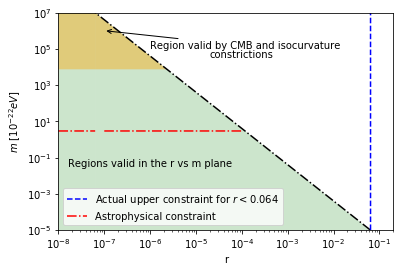
\includegraphics[width=8cm]{SFDMconstraints.png}
\caption{Isocurvature constraints for the SFDM candidate.
%\jav{ya me confundio esta figura. Seria bueno poner los ejes al reves, ya que $r$ se esta buscando 
%y $m$ seria un derivado. De acuerdo a esta figura, cuales son las constricciones actuales a la masa?}
%\jav{quitar la flecha y mejor centrar el texto, explicar regiones.}
}\label{constraintsSFDM}
\end{figure}
%%%%-------------------------------------------------------------------------------------------%%%
%\begin{center}
\subsection{Real Self-interacting SFDM Candidate}
\subsubsection{Cosmological history}
%\end{center}0
%%%-------------------------------------------------------------------------------------------%%%

In this section a self-interacting SFDM with a positive interaction is considered. This scenario is described by the general potential
\begin{equation}
V(\phi,|\psi|^2)=V(\phi)+\frac{1}{2}m^2\psi^2+\frac{1}{4}\lambda\psi^4,
\end{equation}
and fixing again $Q=0$ for the SFDM in equation [14].

Notice that for this case $M^2=m^2+\lambda\psi^2$. 
%\jav{se vale? ya que $\psi$ 
%evoluciona, y por tanto la masa también}\lp{Yo le llam ́e masa efectiva,
%pero no es realmente una masa}. 
As we have previously discussed the effective mass of the field after inflation remains 
constant at $M^2=m^2+\lambda\psi_i^2$ until $M\sim H$. Then, depending of each contribution to $M^2$, we can 
have two different dynamics. 
\\

%%%-------------------------------------------------------------------------------------------%%%
\textbf{\textit{Weakly self-interacting regime.-}} This limit is obtained when the constant term $m^2$ dominates, 
that is when
%
\begin{equation}\label{consw}
m^2\gg \lambda\psi_i^2.
\end{equation}
In this regime it is possible to ignore the autointeracting term in equation \eqref{KGe3} when the oscillations 
of the scalar field begins. 
However, by ignoring this term the field behaves as a massive field and from
\eqref{rhosfdm} the field value always decreases. Therefore the autointeracting term never dominates and 
all the cosmological history remains the same as in the pure massive SFDM scenario.  In fact, thanks to the 
decreasing behavior of this scenario we can consider that this regime is fulfilled always that 
$m^2\geq \lambda|\psi_i|^2/2$ or equivalently when $\lambda\leq 2m^2/|\psi_i|^2$. 
%
If the SFDM oscillations start at the same time than the massive case (which is a good approximation since the effective mass of the SFDM is $M^2 =m^2 +\lambda\psi^2_i \leq 2m^2$), 
%\jav{por que es una buena aproximacion?}\lp{Por lo que agregu\'e en los par\'entesis} 
we observe from \eqref{phi_im2} that it must be fulfilled that
%
\begin{equation}
\left(\frac{\lambda}{10^{-96}}\right)\leq 1.2\left(\frac{m}{10^{-22}eV}\right)^{5/2}.
\end{equation}
%\jav{estamos hablando del strong or weakly scenario? porq la ecuacion que usas se basa en el weakly scenario!!} 
We plot in figure \ref{weekregime} the weak limit obtained by our approximation. However this 
overestimates the maximum value of $\lambda$ since the dust-like behavior is obtained when the $\lambda$ term is completely negligible.%
\begin{figure}[h!]
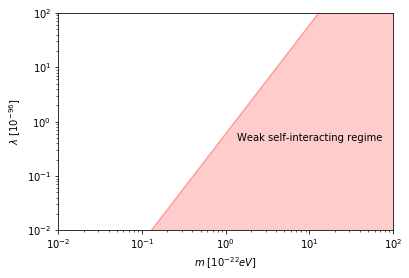
\includegraphics[width=8cm]{weakregime.png}
\caption{Weakly self-interacting regime}
\label{weekregime}
\end{figure} 


%%%-------------------------------------------------------------------------------------------%%%
\textbf{\textit{Strong self-interacting regime.-}} This scenario is obtained when 
\begin{equation}
m^2\ll \lambda\psi_i^2.
\end{equation}
%
Here the SFDM follows an attractor solution during the inflationary era.
\\

%%%-------------------------------------------------------------------------------------------%%%
\textit{Attractor behavior of the SF during inflation.-} In the strong self-interacting regime the SFDM follows the 
attractor solution \cite{curvatonatractor}\footnote{The study done in reference \cite{curvatonatractor} 
was for a curvaton-like scalar field in a chaotic-like inflationary scenario. However their results can 
be used as well in this context were the attractor behavior can be easily obtained for whichever inflationary potential.}
\begin{equation}\label{atractor}
\psi_{att} =\left(2\lambda\int_{\phi}^{\phi_0}V^{-1}_{,\phi}d\phi\right)^{-1/2},
\end{equation}
where $\phi_0$ is the value of the inflaton at the beginning of inflation. 
In the above expression we can identify two possible branches:
\begin{itemize}
\item $\psi_{att}<\sqrt{2}m/\sqrt{\lambda}$

The SFDM follows the attractor solution until $\psi\simeq \sqrt{2}m/\sqrt{\lambda}$. Then the field 
reaches $\psi_i=\sqrt{2}m/\sqrt{\lambda}$ for the rest of inflation. Notice that this value corresponds to the upper 
limit that the weakly self-interacting regime allows. 
%
Then the field starts evolving when $H\sim M\simeq m$ behaving as a massive SF. In this way the constrictions 
given in the non-interacting case apply and the initial conditions are also fixed by $\psi_i$. 
Using both relations the $\lambda$ value is approximated 
%to \jav{la eqn lleva un $\sim$ en lugar de $=$?}\lp{Tienes raz\'on, ya lo cambi\'e}
%
\begin{equation}\label{wregime}
\left(\frac{\lambda}{10^{-96}}\right)\simeq 1.2\left(\frac{g_{*osc}}{3.36}\right)^{3/4}\left(\frac{g_{s*osc}}{3.91}\right)^{-1}\left(\frac{m}{10^{-22}eV}\right)^{5/2}.
\end{equation}
%
The mass term and the auto-interacting constant are rescaled by appropriate values, that is, the mass term is measured 
in units of $10^{-22}eV$ while the auto-interacting constant in terms of $10^{-96}$ \jav{unidades}\lp{Seg\'un yo es adimencional.}.
\\

\item $\psi_{att}>\sqrt{2}m/\sqrt{\lambda}$

In this scenario the dynamics of the inflaton, given by \eqref{atractor}, implies that the initial condition 
of the field after the inflationary period is
%
\begin{equation}\label{atractor2}
\psi_{att}^i = \left(2\lambda\int_{\phi_{end}}^{\phi_0}V^{-1}_{,\phi}d\phi\right)^{-1/2},
\end{equation}
%
where $\phi_{end}$ is the value of the inflaton at the end of inflation. 
We need to stress out that this is the value of the field until its oscillation period starts (i.e. when $M\sim H$).

In this scenario we observe that at the time the SFDM starts its oscillations its effective mass is quadratic in the field. 
In that regime the scalar field evolves as $\psi\sim 1/a$ and its energy density as $\rho_{\psi}\sim 1/a^4$, 
behaving as radiation. Then, when $m^2 \sim \lambda\psi_t^2$ the effective scalar field mass is now constant, 
obtaining the dust-like behavior already analyzed. 
Therefore, the history of the scalar field density is
%
\begin{equation}\label{rhosfdmlam}
\rho_\psi = \left\lbrace\begin{array}{ll}
\frac{1}{4}\lambda^2\psi_i^4 & \text{when }H\gg \lambda\psi_i^4 \\
\frac{1}{4}\lambda\psi_i^4\left(\frac{a_{osc}}{a}\right)^4 & \text{when }H_t\leq \lambda\psi_i^4\leq H\\
\frac{1}{2}m^2\psi_t^2\left(\frac{a_t}{a}\right)^3 & \text{when } H\leq m^2\ \text{and}\ \lambda\psi^2<m^2
\end{array}\right .
\end{equation}
%
Here sub-index $t$ means quantities measured at transition between radiation-like to dust-like behavior of the SFDM and
\begin{equation}\label{inilamb}
\psi_i^2=\left[\frac{2m^2}{\lambda}\psi_t^2\right]^{1/2}\left(\frac{a_t}{a_{osc}}\right)^2.
\end{equation}
%
Notice that, for simplicity, we have taken an instantaneous transition between radiation-like to dust-like behaviors. 

%In order to continue it is necessary to specify the value of $a_t$ and $a_s$. 
Since the auto-interacting KG equation cannot be solved exactly we work with approximated 
solutions. 
%\jav{y numericamente?}\lp{pongo que s\'i se  podr\'ia,  pero  lo  que  me  interesa  es  obtener  la condici\'on inicial $\psi_i$ del campo escalar y obtenerlo como funci\'on de $\lambda$ y $m$. Se me hace mucho m\'as f\'acil
%utilizar estas aproximaciones semianal\'iticas que andar resolviendo muchas veces el campo escalar para diferentes $\lambda$s y $m$s para luego comparar}. 
By using a pure approximated description of the system,
 \cite{SFphi42} obtained the relation (see its equation 80 and 86 and also \cite{SFphi41})
 \footnote{The reference \cite{SFphi42} obtained this relation by considering a Universe with only a SFDM content. 
 However a similar analysis can be used in a Universe with several types of matter contents.} 
% \jav{si ya lo obtuvieron ellos, que obtienes nuevo?}\lp{Hasta  aqu\'i  nada,  s\'olo  estoy usando su resultado para obtener la condici\'on inicial que ando buscando. Tal vez lo nuevo es que yo ya lo estoy mentiendo considerando que el campo escalar coexisti\'o con el inflat\'on, mientras que la referencia que estoy dando lo estudiaron como lo digo en
%el pie de p\'agina.}
 %
\begin{subequations}
\begin{equation}\label{atoveras}
\left(\frac{a_t}{a_{osc}}\right)^2=\frac{3}{7^{1/3}f^2(\frac{a_s}{r_S})},
\end{equation}
where 
\begin{equation}
f(\sigma)=\frac{1}{s^{1/3}(1+4s)^{1/6}},
\end{equation}
with
\begin{equation}
s=\frac{4\sigma-1+\sqrt{(4\sigma-1)^2+12\sigma}}{6}.
\end{equation}
\end{subequations}
%
Additionally $r_S=2mG/c^2$ and $a_s=\hbar^2\lambda/4\pi m$. 
Then it follows that $a_s/r_S=\lambda M_p^2/m^2$. 
Rearranging the expression in a more convenient way we have
\begin{equation}
\sigma \simeq 5.93\times 10^{
2}\left(\frac{m}{10^{-22}eV}\right)^{-2}\left(\frac{\lambda}{10^{-96}}\right).
\end{equation}
%

Notice that when $a_t/a_{osc}\simeq 1$, i.e.  $3/(7^{1/3}f^2(\sigma))\sim 1$, there is no radiation-like epoch. 
This scenario should match with the non-interacting scenario that we present previously.  Inserting equation \eqref{atoveras} into \eqref{inilamb} yields to
\begin{equation}\label{inilamb2}
\psi_i^2=\frac{3}{7^{1/3}f^2(\sigma)}\left[\frac{2m^2}{\lambda}\psi_t^2\right]^{1/2}.
\end{equation}
%

The relation (\ref{inilamb2}) matches the field at $\psi_t$ with its value right after inflation ends. 
Then if we obtain the value of $\psi_t$ by comparing with quantities at present, with the above expressions 
we can also obtain the value of $\psi_i$. On the other hand, notice that at $a_t$ the scalar field behaves 
as dust with an effective mass $M^2=m^2+\lambda\psi^2_t$. This implies that dust-like oscillations 
of the SF began a little before than in the non-interacting case. If we allow $m$ to be 
ultra-light ($m\sim 10^{-��22}eV$) and using the fact that $m^2$ is about the same 
order that $\lambda\psi^2_t$, 
%\jav{de donde se ve esto?}\lp{Anteriormente defin\'i $\psi_t$ 
%como el valor del campo donde se cumple que $m^2\sim \lambda\psi^2_t$} 
we get that such oscillations start during the same epoch 
than in the non-interacting case. 
%
In fact because the decreasing behavior of the SF during the dust-like period 
%\jav{which period}\lp{Cuando comienzas las dust-like oscillations} 
($\psi\sim 1/a^{3/2}$) the auto-interacting term contribution quickly vanishes and then the dynamics of the field is described  only by the mass term $m$. Thus, once the dust-like behavior starts, the dynamics 
is described similarly to  the non-interacting case, in such case the condition \eqref{phi_im2} is fulfilled by 
the SF as well, but interchanging subindex $i$ with $t$\footnote{In fact this is a lower limit for the 
strong auto-interacting case.}.
%\jav{creo que las ideas estan un poco mezcladas, por que al final siempre terminas con la contribucion $m^2\phi^2$}\lp{Siempre debo terminar con esa contribuci\'on porque al final necesito  que  el  campo  escalar  se  comporte  como polvo.  Entonces lo  \'unico que estoy haciendo aqu\'i es  obtener  cual  es  la  contribuci\'on  de  la  ́\'epoca  de
%radiaci\'on.   Digo  que  durante  el  per\'iodo  de  polvo se  cumple  lo  que  ya  hab\'iamos  obtenido  para  un campo masivo y eso lo uso junto con la ecuaci\'on 27 y 28a para obtener la contribuci\'on que da la  \'epoca de radiaci\'on y con ello la condici\'on inicial durante inflaci\'on}
\end{itemize}
%%%=========================================================================%%%
\subsubsection{Constraints from isocurvature perturbations}
%%%=========================================================================%%%

As we have shown in the last section we have two different scenarios for this model: 
a weak self-interacting and a strong self-interacting. In the weak limit our SFDM behaves 
effectively as a massive field without auto-interaction, and in such case the constrictions 
for the massive field apply to this scenario as well. On the other hand when the auto-interacting 
term is big enough, the SFDM will have a new period with a behavior similar to a radiation-like fluid. 
In this way the constrictions we obtained before will not apply to this model anymore 
\\
%\jav{por que?}
%\jav{osea que el weak interacting, no aporta nada?}\lp{El weak interacting es b\'asicamente de nuevo el campo masivo, mientras que en el otro ya tenemos un per\'iodo en el que el SFDM se comporta diferente}.

%Before studying the strong scenario notice that we can give general constrictions for the 
%auto-interacting contribution in terms of our previous expressions. 

In the strong self-interacting regime, during the inflationary era, the SFDM follows the attractor solution \eqref{atractor}.
%\begin{equation}\label{atractor0}
%\psi_{att} =\left(2\lambda\int_{\phi}^{\phi_0}V^{-1}_{,\phi}d\phi\right)^{-1/2}
%\end{equation}
The value that the homogeneous field acquired  after inflation depends on the condition 
$\psi_{att}\lessgtr \sqrt{2}m/\sqrt{\lambda}\equiv \psi_t$. 
For $\psi_{att}<\psi_t$ the field follows the attractor solution until $\psi\simeq \psi_t$. 
Then the SFDM is frozen at that value and starts oscillating as a massive field 
when $m\sim H$. We can constraint this scenario by noticing that it is the same than the massive case but with the initial condition $\psi_i=\psi_t$.  Matching Eq. \eqref{phi_im2} with $\psi_t$ and making use of the constriction \eqref{constm} we obtain
%
\begin{equation}
\left(\frac{\lambda}{10^{-96}}\right)\leq 1.2\left(\frac{2\times 10^{-4}}{r}\right)^5.
\end{equation}
In figure \ref{constraintsSFDMl} we have plotted the above condition that is valid during the strong 
%\jav{weak? sure? al inicio del parrafo dice strong}\lp{Me equivoqu\'e, ya lo correg\'i} 
self-interacting regime, when $\psi_{att}<\psi_t$. 
The  pink  region corresponds to the region allowed by isocurvature perturbations in this limit.  
As we  observe the self-interacting term for this model can be constrained in a similar way than the 
mass parameter in the massive case. 
This scenario must fulfill the relation \eqref{constm} as well, since its cosmological evolution after inflation is only like a massive SFDM.

\begin{figure}[h!]
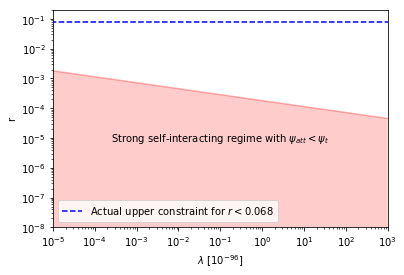
\includegraphics[width=8cm]{lambdavsr.png}
\caption{Isocurvature constraints for the strong self-interacting regime with $\psi_{att}<\psi_t$.}\label{constraintsSFDMl}
\end{figure} 

Additionally, in this scenario, the inflationary potential fulfills the condition 
%
\begin{equation}
\left(\int^{\phi_0}_\phi V_{,\phi}^{-1}d\phi\right)^{-1/2}<2m.
\end{equation}
%
We can see that it is very difficult to obtain this relation for an ultra-light SFDM candidate. 
For example, if we consider a chaotic-like inflationary potential, $V(\phi)=\frac{1}{2}M_{inf}^2\phi^2$, 
the above conditions implies that
%
\begin{equation}\label{chaoticweek}
\left(\log\frac{\phi_0}{\phi}\right)^{-1/2}<2\frac{m}{M_{inf}}.
\end{equation}
%
However, for this potential the mass $M_{inf}$ of the inflaton 
that best matches the observations\footnote{This chaotic-like inflationary potential is 
ruled-out now for observations, however we use it as an example in order to obtain 
general constraints for our models.} is of order $M_{inf}\sim 10^{12} GeV$ \cite{Liddle}. 
If now we assume an ultra-light SFDM candidate with a mass $m\sim 10^{-22}eV$, 
the above conditions implies that the logarithmic part of the expression should be 
lower that $\sim 10^{-43}$. The inflationary behavior for a chaotic-like inflaton ends 
when $\phi_{end}\simeq 2M_{pl}$ \cite{curvatonatractor,Liddle}. Moreover as it is 
explained in \cite{curvatonatractor}, the initial condition of the inflaton cannot be 
arbitrarily large since the stochastic behavior is significant for $\dot\phi H^{-1}<H/2\pi$. 
%
If the Universe starts when the inflaton escapes from this 
behavior we have that its initial condition should be
%
\begin{equation}\label{phi_0}
\phi_0\sim 10^5\times M_{pl}\left(\frac{10^{13}GeV}{M_{inf}}\right)^{1/2}.
\end{equation}
%
where we can easily see that the condition given in \eqref{chaoticweek} cannot be fulfilled. 
%\jav{y si no se satisface, que pasa?}\lp{No podr\'ia estar el campo escalar auto-interactuante en
%el r\'egimen d\'ebil con el inflat\'on.  Esto no representa un
%gran problema ya que entonces significar\'ia que el campo
%escalar deber\'ia estar en el r\'egimen fuerte}. 
This implies that if we consider that an ultra-light self-interacting SFDM candidate coexists with the inflaton, 
it should be within the strong regime since their conditions are easier to satisfy.

When $\psi_{att}>\psi_t$ we have that the field follows the attractor solution during all the inflationary period. 
Hence the initial condition for the SFDM is given by \eqref{atractor2}
%
\begin{equation}\label{atractor3}
\psi_{att}^i = \left(2\lambda\int_{\phi_{end}}^{\phi_0}V^{-1}_{,\phi}d\phi\right)^{-1/2}.
\end{equation}
%
Then the SFDM remains frozen at value $\psi_{att}^i$ until $M\sim H$ and starts oscillating with a 
quartic potential. In this scenario the SFDM density behaves as $\rho_{SFDM}\propto \psi^4$ and 
in such case we can write $\delta\rho_{\psi}/\rho_\psi=4\delta\psi/\psi_i$. Therefore the primordial 
isocurvature perturbations for a strong self-interacting SFDM is given by
%
\begin{equation}
P_{SFDM}(k)=\left(\frac{2H_*}{\pi\psi_i}\right)^2.
\end{equation}
%
In the last section we showed the relation of the initial condition  with the value of the 
field today. Using eqs. \eqref{inilamb2} and \eqref{phi_im2}, 
with $g_{*osc}=3.36$ and $g_{s*osc}=3.91$  and considering appropriate units we obtain
%
\begin{equation}\label{constr4}
r<\frac{1.172\times 10^{-4}}{7^{1/3}f^2(\sigma)}\left[\frac{2
\left(\frac{m}{10^{-22}eV}\right)^{3/2}}{\left(\frac{\lambda}{10^{-96}}\right)}\right]^{1/2}.
\end{equation}
%
Similarly to the the massive case, the above relation must be compared with observations in order to get constrictions for  the
strong self-interacting SFDM scenario. 
%However in the literature we reviewed we couldn't find so much constrictions for the self-interacting regime. Then, let us review what we found. 
\\


\textit{Other constraints}.- In \cite{constl1} it was studied the possibility that a SFDM candidate could be self-instarcting. In their work they constraint the ratio $\Lambda\equiv m/\lambda^{1/4}$ to be $\Lambda\sim 1eV$ by analyzing the line-of-sight velocity dispersion for the eight dSphs satellites of the Milky Way (MW). This study was complementary to the ones done in \cite{constl2,constl3,constl4,constl5} where the SFDM model was studied by employing rotational curves of the most Dark Matter domminated galaxies from different surveys and where they obtained the constriction $\Lambda\sim 2.6-2.9eV$. On the other hand, in \cite{constl6} the model was studied in a cosmological context by demmanding that the SFDM candidate behaves as a dust-like component before the time of matter-radiation equality. In such work they obtain the result $\Lambda>0.8eV$. Finally, it was also possible to test the self-interacting scenario by considering the number of extra relativistic species at BBN. When such observations are confronted with the SFDM it is obtained that it must be filfilled that $\Lambda\gtrsim 4eV$ (see \cite{constl3}).    

%To test the model at galactic levels we assume the ground state of the SFDM 
%corresponds to the minimum galaxy halo (i.e. Fornax) \cite{SFphi42}, then it is possible to constrain the ratio $%\lambda/m^2$. 
%Also, if we use observations coming from the Bullet Cluster \cite{bullet} it is possible to limit one of the parameters of the model. 
%\jav{no entendi}\lp{Quiero decir que con FORNAX se obtiene el radio entre $\lambda$ y $m$ y con bullet cluster se fijan los valores que $m$ y $\lambda$ deben tene}. 
%In \cite{SFphi42} it was obtained that for a strong self-interacting SFDM model we have
%
%\begin{equation}
%m\simeq 1.10\times10^{-3}eV, \ \ \ \ \lambda \simeq 2.46\times 10^{-17},
%\end{equation}
%
%This result corresponds to the upper bound of the mass of the SFDM while the non-interacting 
%case should corresponds with the lower bound. Therefore the mass of the SFDM should be in the 
%range $2.92\times 10^{-22}\lesssim m\lesssim 1.10\times 10^{-3}eV$ while the self-interacting 
%term in the range $0\lesssim \lambda \lesssim 1.69\times 10^{-17}$. On the other hand when 
%the model is tested at cosmological levels using the CMB and the 
%abundances of light elements produced by the BBN it is obtained the values \cite{SFphi41,SFphi42}
%
%\begin{equation}\label{masslamb}
%m\simeq3\times 10^{-21}eV, \ \ \ \ \ \lambda \simeq 1.69\times 10^{-87}.
%\end{equation}
%
%Notice that these expressions are in agreement with the ones given by galactic constrictions.
%
%Considering \eqref{masslamb} as the most acceptable values for the mass of the SFDM and 
%its auto-interacting term we can easily see from Figure \ref{weekregime} that we should be in the strong regime. 
%Then in this scenario the constrictions given in Eq. \eqref{constr4} should apply. 
%
In figure \ref{constraintsSFDMls} we have plotted contour levels of the numerical value of the right side of the relation \eqref{constr4}. 
The grey region corresponds to values larger than $0.064$ which is the actual upper constraint on tensor-to-scalar ratio. 
This means that within that region we are certain that \eqref{constr4} is fulfilled and, by the moment, just this region is completely allowed by observations. With this in mind the plot should be understood as follows: lets suppose that in the near future we meassure a value for $r$. Such value will coincide with a curve in figure \ref{constraintsSFDMls}. Then, the space of parameters that could continue be allowed by data should be the one where the contour levels are bigger than the detected value of $r$, while the one with an smaller value in the contour levels must be discarded. Similarly than in the massive case, if $r$ is not detected but it continue being constrained with an upper limmit, this implies that the regions with contour levels bigger than such upper value will be allowed by the data, but the regions with smaller values can not be discarded until $r$ is detected.

The value of $\Lambda$ that fulfil observations of dSph's Light-of-sight is given by the dot-dashed red line, while the region of parameters neccesary for rotational curves is presented in blue. Simmilar than in the massive plot (fig. \ref{constraintsSFDM}) we plotted the cosmological constriction in purple by drawing a curve that refers to the upper value of $\Lambda$ and an arrow that point out the region that remains valid for the constriction. We did the same for the observations for BBN but in fuchsia. The white region corresponds to the weak limit.  
We can see from figure \ref{constraintsSFDMls} that it is possible to fulfill observations for whichever value for the mass as long as the self-interacting constant is large enough. In other words, for a given mass, the measurement of $r$ can only constraint the self-interacting constant with a lower limmit. Isocurvature observations (or equivalently onservations on $r$) can also help the model to constraint with an upper value other observations. As an example lets suppose that we want to be completely sure that the meassurements obtained by rotational curves are fulfilled. Then, given the actual upper constraints in $r$ , the only region of parameters that we can be sure that fulfil observations are the ones in the blue region that are also inside the gray region. 
%
\begin{figure}[h!]
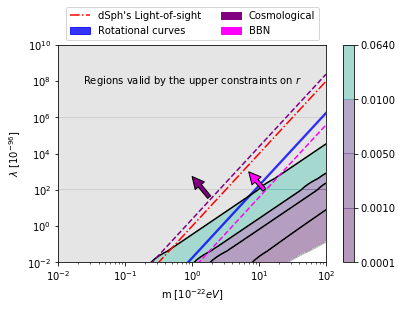
\includegraphics[width=8cm]{stronglamb.png}
\caption{Isocurvature constraints for the strong self-interacting scenario with $\psi_{att}>\psi_t$.
}\label{constraintsSFDMls}
\end{figure} 

Remark: This scenario is of special interest given that the attractor solution justify the initial 
conditions for the SFDM model and because it is natural to avoid isocurvature perturbations 
when the auto-interacting term of the SF is big enough.
 \\

Similarly to the above description we can compute general constraints for the inflationary 
potential that should generate inflation on these kind of scenarios. First we have that
%
\begin{equation}
\left(\int^{\phi_0}_\phi V_{,\phi}^{-1}d\phi\right)^{-1/2}>2m,
\end{equation}
%
which is very easy to fulfill as we saw in the chaotic-like example. Using isocurvature constriction we also have
%
\begin{equation}
r<\frac{0.6\times 10^{40}}{\left(\frac{\lambda}{10^{-96}}\right)}\left(\frac{1}{\int_{\phi_{end}}^{\phi_0}V_{,\phi}^{-1}d\phi}\right),
\end{equation}
%
that can also be satisfied as far as the auto-interacting term and the integral are small enough; 
for example in the chaotic-like scenario by using \eqref{chaoticweek} and \eqref{phi_0}
%\begin{equation}
%\left(\int^{\phi_0}_\phi V_{,\phi}^{-1}d\phi\right)^{-1/2}\simeq (0.7403)\times 10^{21}
%\end{equation}
and taking $M_{inf}\simeq 10^{-6}M_{pl} $, we can obtain the constriction 
%
\begin{equation}
\left(\frac{\lambda}{10^{-96}}\right)<\frac{0.3288\times 10^{84}}{r}.
\end{equation}
that is easily satisfied for whichever value of $\lambda$ of our interest.
%
%
If now we compare \eqref{atractor2} and \eqref{inilamb2} we have
%
\begin{equation}\label{inilamb3}
\left(\int_{\phi_{end}}^{\phi_0}V^{-1}_{,\phi}d\phi\right)^{-1}=\frac{6}{7^{1/3}f^2(\sigma)}\left(2m^2\lambda|\psi_t|^2\right)^{1/2}.
\end{equation}
This relation is interpreted as follows: consider that the auto-interacting SFDM candidate 
coexists with the inflaton, and suppose there are several measurements constraining the mass 
parameter $m$ as well as the auto-interacting parameter $\lambda$, therefore such constraints are translated into 
restrictions to the inflationary potential.  

It is also necessary to be careful that the SFDM does not come to dominate the inflationary period. 
%\jav{por que?}\lp{Si domina tendr\'iamos que considerar inflaci\'on
%de 2 campos.  Adem\'as tendr\'iamos que justificar como es
%que le hizo el campo escalar para luego volverse subdominante y volver a dominar en igualdad materia-radiaci\'on}.  
This is guarantee by demanding that
%
\begin{equation}
\lambda < \frac{H_*^2 M_p^2}{|\psi_i|^4},
\end{equation}
%
or in terms of \eqref{atractor3}
%
\begin{equation}\label{constd}
\lambda>\left(4H_*^2M_{pl}^2\left(\int_{\phi_{end}}^{\phi_0}V_{,\phi}^{-1}d\phi\right)^2\right)^{-1}.
\end{equation}
%
Taking the chaotic-like example and using $H_*= 10^{14} GeV$, we obain the constriction
\begin{equation}\label{lowerlambda}
\frac{\lambda}{10^{-96}} > 5.777\times 10^{77}.
\end{equation}
Notice that the above expresion requires that $\lambda>10^{-19}eV$. We have to stress out that \eqref{lowerlambda} is obtained for a  chaotic-like potential, then, depending the inflationary potential we will have different limmit allowed for the self-interacting scenario. On the other hand if equation \eqref{constd} is not fulfilled and we remain in the strong-self interacting model it should be neccesary to consider a two-field inflationary scenario where the SFDM could obtain a non-negligible dynamycs during inflation.



%\begin{center}
%%%-------------------------------------------------------------------------------------------%%%
\subsection{Complex SFDM generalization}
%%%-------------------------------------------------------------------------------------------%%%
%\end{center}
% A massive complex scalar field is described by the potential
%\begin{equation}
%V(|\psi|^2)= m^2|\psi|^2
%\end{equation}


As we have seen at the beginning of this section, when we consider a complex scalar field its dynamics is modified 
only by the centrifugal term (see eq. \eqref{KGe3}). However as it was mentioned in \cite{SFphi42} 
such term does not affect the dynamics of the field at cosmological levels, obtaining then that a 
complex scalar field and a real scalar field have the same cosmological history in the Universe. 
%
In this way if we take that our complex SFDM fulfill slow-roll conditions during inflation then its 
constrictions for isocurvature perturbations must be the same than in the real field analogue. \\

\section{Discusions and conclusions}\label{conclusions}

In this paper we have studied the possibility that a massive or a self-interacting SFDM particle could coexist with the inflaton during inflation. In our assumptions we have considered the SFDM as an spectator in the inflationary process. Then, the SFDM contributes to the primordial spectrum by generating isocurvature perturbations. By using the actual upper constraint in the measurement of the tensor-to-scalar ratio $r$ it was possible to test the free parameters for each model. However, as we discussed it is not possible for the momment to ruled-out a region of parameters given that it could be only possible to do it if $r$ is meassured.   

Our main result are shown in figures \ref{constraintsSFDM} and \ref{constraintsSFDMls}. In figure \ref{constraintsSFDM} we have identified the masses allowed in the massive model by isocurvature as well as cosmological and astrophysical observations. We obtained that in order to fulfil at least the constrictions impossed by CMB we should not detect gravitational waves until $r\simeq 1.3\times 10^{-3}$, while if we were interested in fulfilling all the observations, we should not detect gravitatinal waves until $r\lesssim 2.33\times 10^{-5}$. This last result is important given that the detectability of gravitational waves could represent a strong constriction for the massive model. Analogously, in figure  \ref{constraintsSFDMls} we have plotted in a $m\ vs\ \lambda$ plane the region of parameters for the strong-self-interacting model that are allowed by observations. What we noticed is that for a given mass of the SFDM it is always possible to avoid isocurvature constrictions and fit astrophysical and cosmological observations if a large enough self-interaction is added. Then we make notice with this result that the addition of a self-interacting component to the SFDM seems to be a natural solution for option in the model given that with this it is possible to filfill naturaly all the constrictrions that the model has. On the other hand we explain the way the SFDM spectator scenario could help to choose the inflationary potential responsible to produce the inflationary period.

%\begin{center}
%\end{center}

\appendix

%\section{•}

\begin{thebibliography}{9}
\bibitem{const1}  P. A. R. Ade
et al.
(Planck), Astron. Astrophys.
571
, A16 (2014), arXiv:1303.5076 [astro-
ph.CO]
\bibitem{const2} ]  P. A. R. Ade
et al.
(Planck), Astron. Astrophys.
571
, A22 (2014), arXiv:1303.5082 [astro-
ph.CO]
\bibitem{planck} P. A. R. Ade et al. (Planck); DOI: 	10.1051/0004-6361/201525898;  	arXiv:1502.02114 [astro-ph.CO]
\bibitem{planck2} P. A. R. Ade et al. (Planck); arXiv:1807.06211 [astro-ph.CO]
\bibitem{const3}  D. Barkats
et al.
(BICEP1), Astrophys. J.
783
, 67 (2014), arXiv:1310.1422 [astro-ph.C]
\bibitem{const4} P. A. R. Ade
et al.
(BICEP2, Planck), Phys. Rev. Lett.
114
, 101301 (2015), arXiv:1502.00612
[astro-ph.CO]
\bibitem{const5}  P.  A.  R.  Ade
et al.
(BICEP2,   Keck  Array),  Phys.  Rev.  Lett.
116
,  031302  (2016),
arXiv:1510.09217 [astro-ph.CO]


\bibitem{SF1} Baldeschi M., Gelmini G., Ruffini R., 1983, Phys.Lett.B, 12.
\bibitem{SF2} Matos T., Guzman F. S., 2000, Class. Quant. Grav. 
\bibitem{SF3} Hu W., Barkana R., Gruzinov A., 2000, Physical Review Letters, 85, 1158.
\bibitem{SF4}Bray H., 2010.
\bibitem{SF5}Schive H.-Y., Chiueh T., Broadhurst T., 2014a, Nature Phys., 10, 496.
\bibitem{SF6}B\"ohmer C. G., Harko T., 2007, J. Cosmology Astropart. Phys., 6, 025.
\bibitem{SF7}Marsh D. J. E., Ferreira P. G., 2010, Phys. Rev. D, 82, 103528.
\bibitem{SF8} Membrado M., Pacheco A. F., Sa\~nudo J., 1989, Phys.Rev.A, 39, 4207.
\bibitem{LCDM1}Peebles P. J. E., 1982, ApJ, 263, L1.
\bibitem{LCDM2}White S. D. M., Frenk C. S., Davis M. et al., 1987, ApJ, 313, 505.
\bibitem{problem1}Bullock J. S., Boylan-Kolchin M., 2017, ARA$\&$A, 55, 343.
\bibitem{problem2}Clowe D., Bradac M., Gonzalez A. H. et al., 2006, ApJ, 648, 2.
\bibitem{problem3}Klypin A., Kravtsov A. V., Valenzuela O. et al., 1999, ApJ, 522, 82.
\bibitem{problem4}Moore B., Ghigna S., Governato F. et al., 1999, ApJ, 524, L19.
\bibitem{problem5}Penny S., Conselice C. J., De Rijcke S. et al., 2009, MNRAS, 393, 1054.
\bibitem{SF9} J. Maga\~na and T. Matos,  Journal of Physics: Conference Series, Volume 378, conference 1.
\bibitem{SF10}  A. Su\'arez, V. H. Robles, and T. Matos, Astrophys. Space
Sci. Proc.
38
, 107 (2014), 1302.0903.
\bibitem{SF11} Marsh D. J. E., 2016, Phys. Rep., 643, 1.
\bibitem{SF12}  L. Hui, J. P. Ostriker, S. Tremaine, and E. Witten, Phys. Rev. D
95
, 043541 (2017).
\bibitem{laldm}L. Visinelli,
Phys. Rev. D 96, 023013 (2017).
\bibitem{twofields} Christian T. Byrnes, David Wands;  Phys.Rev. D74 (2006) 043529; DOI:  	10.1103/PhysRevD.74.043529;  arXiv:astro-ph/0605679v3
\bibitem{infm}J. Alberto V\'azquez, Luis E. Padilla, Tonatiuh Matos, Inflationary Cosmology: From Theory to Observations,  	arXiv:1810.09934 [astro-ph.CO].
\bibitem{H1}  D. Lyth, Physics Letters B
147
, 403  (1984).
\bibitem{H2}  D. H. Lyth and E. D. Stewart, Physics Letters B
283
, 189  (1992).
\bibitem{madelung}  E. Madelung, Zeit. F. Phys.
40
, 322 (1927).
\bibitem{SFphi41}  B. Li, T. Rindler-Daller, and P.R. Shapiro, Phys. Rev.
D
89
, 083536 (2014).
\bibitem{SFphi42} A. Su\'arez and P. H. Chavanis,
Phys. Rev. D
95
, 063515
(2017)
.
\bibitem{charge1} A. Su\'arez and P.H. Chavanis, Phys. Rev. D
92
, 023510
(2015).
%\bibitem{charge2} \textcolor{red}{ B. Li, T. Rindler-Daller, and P.R. Shapiro, Phys. Rev.
%D
%89
%, 083536 (2014)}
\bibitem{charge3}  A. Arbey, J. Lesgourgues, and P. Salati, Phys. Rev. D 65, 083514 (2002).
\bibitem{charge4}  J.-A.  Gu  and  W.-Y.P.  Hwang,  Phys.  Lett.  B
517
,
(2001).
\bibitem{atractorinf1}  V.A.  Belinsky,  L.P.  Grishchuk,  I.M.  Khalatnikov,  and
Ya.B. Zeldovich, Phys. Lett. B
155
, 232 (1985).
\bibitem{atractorinf2}  T.  Piran  and  R.M.  Williams,  Phys.  Lett.  B
163
,  331
(1985).
\bibitem{SFrev2}T. Kobayashi, R. Murgia, A. De Simone, V. Ir\~si\~c, and M.
Viel,
Phys. Rev. D
96
, 123514 (2017).
\bibitem{curvatonatractor}   K. Harigaya, M. Ibe, M. Kawasaki and T. T. Yanagida, Phys. Rev. D
87
, 063514
(2013) [arXiv:1211.3535 [hep-ph]].
\bibitem{constn1}Hlozek R., Grin D., Marsh D. J. E., Ferreira P. G., 2015, Phys.
Rev. D, 91, 103512.
\bibitem{constn2}Paredes A., Michinel H., 2016, Physics of the Dark Universe, 12,
50.
\bibitem{constn3} A. X. Gonz\'ales-Morales, D.J.E. Marsh, J. Pe\~narrubia,   and L. Ure\~na-L\'opez, Unbiased constraints on ultralight axion
mass from dwarf spheroidal galaxies, ArXiv e-prints (2016), arXiv:1609.05856.
\bibitem{constn4}Lora  V.,  Maga\~na  J.,  Bernal  A.,  S\'anchez-Salcedo  F.  J.,  Grebel
E. K., 2012, J. Cosmology Astropart. Phys., 2, 11.
\bibitem{constn5}Calabrese E., Spergel D. N., 2016, MNRAS, 460, 4397.
\bibitem{constn6}Sarkar A., Mondal R., Das S., Sethi S. K., Bharadwaj S., Marsh
D. J. E., 2016, J. Cosmology Astropart. Phys., 4, 012.
\bibitem{constn7}Armengaud   E.,   Palanque-Delabrouille   N.,   Y\`eche   C.,   Marsh
D. J. E., Baur J., 2017, preprint,  (
arXiv:1703.09126
).
\bibitem{constn8} Ir\~si\~c  V.,  Viel  M.,  Haehnelt  M.  G.,  Bolton  J.  S.,  Becker  G.  D.,
2017, preprint,  (
arXiv:1703.04683
).
\bibitem{Liddle}D. H. Lyth and A. R. Liddle, \textit{The primordial density perturbation; cosmology inflation and the origin of structure} , 2009, Cambridge University Press.
\bibitem{constl1}Diez-Tejedor A., Gonz\'ales-Morales A. X., Profumo S.,
20014, Phys. Rev. D, 90, 043517, 1404.1054, ADS.
\bibitem{constl2} C.G.  Boehmer  and  T.  Harko,  Can  dark  matter  be
a  Bose-Einstein  condensate?,  JCAP
0706
025  (2007)
[arXiv:0705.4158[astro-ph]].
\bibitem{constl3}  A. Arbey, J. Lesgourgues and P. Salati, Galactic halos
of  fluid  dark  matter,  Phys.  Rev.  D
68
023511  (2003)
[astro-ph/0301533.
\bibitem{constl4} T.  Harko,  Bose-Einstein  condensation  of  dark  matter
solves the core/cusp problem,  JCAP
1105
022 (2011)
[arXiv:1105.2996[astro-ph.CO].
\bibitem{constl5} V.H. Robles and T. Matos, Flat central density profile
and constant DM surface density in galaxies from Scalar
Field  Dark  Matter,  Mon.  Not.  Roy.  Astron.  Soc.
422
282-289 (2012) [arXiv:1201.3032[astro-ph.CO].
\bibitem{constl6} A.  Arbey,  J.  Lesgourgues  and  P.  Salati,  Cosmological
constraints  on  quintessential  halos,  Phys.  Rev.  D
65
083514 (2002) [astro-ph/0112324.


%\bibitem{bullet}  S.W. Randall, M. Markevitch, D. Clowe, A.H. Gonzalez,
%42
%and M. Bradac, Astrophys. J.
%679
%, 1173 (2008)

%\bibitem{princ_ad}P.J.E. Peebles, \textit{Principle of Physical Cosmology} (Princeton University Press, 1993)
%\bibitem{princ_ad2}A. R. Liddle y S. Lyth, \textit{Cosmological inflation and large scale structure} (Cambridge University Press, 2000).
%\bibitem{curvaton2}D.H. Lyth and D. Wands,
%Generating the curvature perturbation without an inflaton
%,
%Phys. Lett.
%B 524
%(2002) 5.
%[
%hep-ph/0110002
%] [
%IN
%SPIRE
%].
%\bibitem{centrif}  J. A.  Gu  and  W.-Y.P.  Hwang,  Phys.  Lett.  B
%517, (2001)
%\bibitem{qsm2} T.  Piran  and  R.M.  Williams,  Phys.  Lett.  B
%163
%,  331
%(1985)

%\bibitem{curvaton13}  D.  H.  Lyth  and  D.  Wands,  Phys.Rev.
%D68
%,  103516
%(2003), astro-ph/0306500
%\bibitem{curv3} T. Moroi and T. Takahashi, Phys. Lett. B
%522
%(2001) 215 [hep-ph/0110096]




%\bibitem{curv1}K. Enqvist and M. S. Sloth, Nucl. Phys. B
%626
%(2002) 395 doi:10.1016/S0550-3213(02)00043-3
%[hep-ph/0109214
%\bibitem{curv2} D. H. Lyth and D. Wands, Phys. Lett. B
%524
%(2002) 5 doi:10.1016/S0370-2693(01)01366-1
%[hep-ph/0110002

%\bibitem{Planckcolaboration}  P.   A.   R.   Ade
%et   al.
%[Planck   Collaboration],    Astron.   Astrophys.
%594
%,    A13   (2016)
%[arXiv:1502.01589 [astro-ph.CO]].
%\bibitem{effdeg}L. Husdal, (2016), 1609.04979.
%\bibitem{massconst1}  P.H. Chavanis, M. Lemou, and F. M ́ehats, Phys. Rev.
%D
%12
%, 123527 (2015)
%\bibitem{curvaton9}T. Moroi and T. Takahashi, Phys. Rev. D
%66
%, 063501 (2002) [arXiv:hep-ph/0206026].
%\bibitem{curvaton10}] D. H. Lyth, C. Ungarelli and D. Wands, Phys. Rev. D
%67
%, 023503 (2003)
%[arXiv:astro-ph/0208055]
%\bibitem{curvaton11} D. H. Lyth and D. Wands, Phys. Rev. D
%68
%, 103516 (2003) [arXiv:astro-ph/0306500].
%\bibitem{curvaton14} C.  He,  D.  Grin  and  W.  Hu,  Phys.  Rev.  D
%92
%,  no.  6,
%063018 (2015), arXiv:1505.00639.%

%\bibitem{curvaton4} D. Langlois and F. Vernizzi,
%Mixed inflaton and curvaton perturbations
%,
%Phys. Rev.
%D 70
%(2004) 063522
%[
%astro-ph/0403258
%] [
%IN
%SPIRE
%].
%\bibitem{curvaton5} T. Moroi, T. Takahashi and Y. Toyoda,
%Relaxing constraints on inflation models with curvaton
%,
%Phys. Rev.
%D 72
%(2005) 023502
%[
%hep-ph/0501007
%] [
%IN
%SPIRE
%\bibitem{curvaton6} T. Moroi and T. Takahashi,
%Implications of the curvaton on inflationary cosmology
%,
%Phys. Rev.
%D 72
%(2005) 023505
%[
%astro-ph/0505339
%] [
%IN
%SPIRE
%].
%\bibitem{curvaton7} K. Ichikawa, T. Suyama, T. Takahashi and M. Yamaguchi,
%Non-Gaussianity, Spectral Index
%and Tensor Modes in Mixed Inflaton and Curvaton Models
%,
%Phys. Rev.
%D 78
%(2008) 023513
%[
%arXiv:0802.4138
%] [
%IN
%SPIRE
%].%

\end{thebibliography}
\end{document}

